% \documentclass[handout]{beamer}
\documentclass[presentation]{beamer}
\usepackage{ctex}
\usecolortheme{duxing}
\usefonttheme{duxing}
\useinnertheme{duxing}

\usepackage[utf8]{inputenc}
\usepackage[UKenglish]{babel}
\usepackage{booktabs}
\usepackage{caption}
\usepackage{subcaption}
\usepackage{graphicx}
\usepackage{amsmath}
\usepackage{amsfonts}
\usepackage{amssymb}

\institute{
\includegraphics[height=0.7cm]{sysu_logo.png}
\includegraphics[height=0.7cm]{duxing_logo.png}}

\title{Python}

\subtitle{如何快速掌握一门编程语言}

\author{陈卓欣}

\date{}


\begin{document}

\frame{\titlepage}

\section{说在前面}

\begin{frame}[standout]
    何为语言?
\end{frame}

\begin{frame}\centering
    1.照样造句
    \par
    2.重复熟练
\end{frame}

\section{基础语法}

\begin{frame}
    \frametitle{语句}\centering
    变量 = 表达式
    \par
    \par
    注意赋值号的理解
\end{frame}

\begin{frame}
	\frametitle{基本结构}\centering
    \begin{columns}
	\column{.4\textwidth}
    顺序结构:\par
    按顺序一句一句往下执行
    \column{.4\textwidth}
    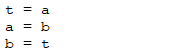
\includegraphics[width=0.75\textwidth]{list.png}
    \end{columns}
\end{frame}

\begin{frame}
	\frametitle{基本结构}\centering
	\begin{columns}
    \column{.4\textwidth}
    分支结构:\par
    判断选择合适的分支\par
    执行相应代码
    \column{.4\textwidth}
    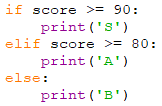
\includegraphics[width=0.75\textwidth]{branch.png}
    \end{columns}
\end{frame}

\begin{frame}
	\frametitle{基本结构}\centering
	\begin{columns}
	\column{.4\textwidth}
    循环结构:\par
    按循环体要求重复执行代码
    \column{.4\textwidth}
    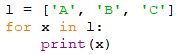
\includegraphics[width=0.75\textwidth]{loop.png}
    \end{columns}
\end{frame}

\section{函数}

\begin{frame}
    \frametitle{函数}\centering
    函数本身是一种表达式\par
    函数也可以组成表达式
\end{frame}

\begin{frame}
    \frametitle{看懂函数}
    语句:变量 = 函数名(参数1,参数2,……)\par
\end{frame}

\begin{frame}
    \frametitle{定义函数}
    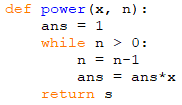
\includegraphics[height=0.4\textheight]{function.png}
\end{frame}

\section{对象}

\begin{frame}
    \frametitle{概念}\centering
    对象是一个抽象概念,\par
    你可以把编程过程中遇到的任何一个“实体”称为对象
\end{frame}

\begin{frame}
    \frametitle{数据类型}
    数:整数、浮点数\par
    逻辑:布尔型\par
    字符:字符串\par
    其他:list,tuple,dict,set,...
\end{frame}

\begin{frame}
    \frametitle{对象的概念}\centering
    \begin{columns}
    \column{.4\textwidth}
    属性:
    对象中的量\par
    语句:类名.属性名
    \column{.4\textwidth}
    方法:
    对象提供的函数\par
    语句:类名.方法名(参数1,参数2,……)
    \end{columns}
\end{frame}

\section{python}

\begin{frame}
    \frametitle{模块}
    python的一大优势\par
    语句:import 模块名\par
    开始愉快地使用模块提供的函数吧!
\end{frame}

\begin{frame}
    \frametitle{关于list}
    列表生成式\par
    生成器与迭代器
\end{frame}

\begin{frame}
    \frametitle{函数式编程}
    把函数也视为“对象”\par
    把函数当作参数或者返回值
\end{frame}

\begin{frame}
    \frametitle{其他}\centering
    正则表达式\par
    异步编程\par
    ……
\end{frame}

\section{说在后面}

\begin{frame}\centering
    1.良好代码风格
    \par
    2.跳出数学思维
    \par
    3.善用搜索引擎
    \par
    4.学好英语
\end{frame}


\begin{frame}[standout]
    Questions
\end{frame}

\end{document}

